\documentclass[letterpaper, 11pt]{article}

\usepackage{lastpage, url, marginnote, siunitx, circuitikz, graphicx, cite, color, textcomp}
% lastpage for couting the total number of pages
% marginnote for putting text in the margin
% textcomp for arrows in texts

\usepackage[margin=1in]{geometry}
%\geometry{hscale=.6, vscale=.8, hmarginratio=2:1, vmarginratio=1:1, marginparwidth=.18\paperwidth, ignoremp}
%\geometry{marginparwidth=.1\paperwidth}

\usepackage{listings}
\definecolor{mygreen}{rgb}{0,0.6,0} \definecolor{mygray}{rgb}{0.5,0.5,0.5} \definecolor{mymauve}{rgb}{0.58,0,0.82}

\lstset{ %
	backgroundcolor=\color{white},   % choose the background color; you must add \usepackage{color} or \usepackage{xcolor}
	basicstyle=\footnotesize,        % the size of the fonts that are used for the code
	breakatwhitespace=false,         % sets if automatic breaks should only happen at whitespace
	breaklines=true,                 % sets automatic line breaking
	captionpos=b,                    % sets the caption-position to bottom
	commentstyle=\color{mygreen},    % comment style
	deletekeywords={...},            % if you want to delete keywords from the given language
	escapeinside={\%*}{*)},          % if you want to add LaTeX within your code
	extendedchars=true,              % lets you use non-ASCII characters; for 8-bits encodings only, does not work with UTF-8
	frame=single,	                   % adds a frame around the code
	keepspaces=true,                 % keeps spaces in text, useful for keeping indentation of code (possibly needs columns=flexible)
	keywordstyle=\color{blue},       % keyword style
	%language=Octave,                 % the language of the code
	otherkeywords={*,...},            % if you want to add more keywords to the set
	numbers=left,                    % where to put the line-numbers; possible values are (none, left, right)
	numbersep=5pt,                   % how far the line-numbers are from the code
	numberstyle=\tiny\color{mygray}, % the style that is used for the line-numbers
	rulecolor=\color{black},         % if not set, the frame-color may be changed on line-breaks within not-black text (e.g. comments (green here))
	showspaces=false,                % show spaces everywhere adding particular underscores; it overrides 'showstringspaces'
	showstringspaces=false,          % underline spaces within strings only
	showtabs=false,                  % show tabs within strings adding particular underscores
	stepnumber=2,                    % the step between two line-numbers. If it's 1, each line will be numbered
	stringstyle=\color{mymauve},     % string literal style
	tabsize=2,	                   % sets default tabsize to 2 spaces
	title=\lstname                   % show the filename of files included with \lstinputlisting; also try caption instead of title
}

\usepackage{enumitem}
\newlist{steps}{enumerate}{1}
\setlist[steps]{label=Step \arabic*, font=\bfseries, leftmargin=-\marginparsep, itemindent=\marginparsep, align=right}

\usepackage{fancyhdr}
\pagestyle{fancy}
\fancyhf{}
\fancyhfoffset[lh,lf]{\dimexpr\marginparwidth+\marginparsep}
\fancyhf[lh]{UCD EEC 134}
\fancyhf[ch]{}
\fancyhf[rh]{}
%\fancyhf[lf]{left foot}
%\fancyhf[cf]{centre foot}
\fancyhf[rf]{Page \thepage /\pageref{LastPage}}
%\renewcommand{\footrulewidth}{.4pt}

%%%%%%%%%%%%%%%
%%%% Tikz definitions
%%%%%%%%%%%%%%%
%\tikzstyle{Uno}=[rectangle,fill=white,draw,line width=0.5mm]

\begin{document}

\title{Appendix A: A Teensy Primer}
\author{Xiaoguang ``Leo'' Liu\\lxgliu@ucdavis.edu}
\date{Last updated: \today}

\maketitle

\section{Introduction}
The Teensy is an open-source 32-bit Cortex-M4 based microcontroller development platform in a very small footprint. All the programming and data connection are done through the USB port; a USB cable with a standard ``Mini-B'' connector is all you need to start using the Teensy!

The Teensy 3.1 features a very capable MK20DX256 32-bit Cortex-M4 processor running at a clock speed of 72 MHz. The MK20DX256 has 256K flash memory, 64K RAM, and 2K EEPROM. The peripherals include 21 analog input, 12 PWM output, 3 UART channels, 2 I2C channels, and 1 SPI channel. Worth noting is that the digital pins are compatible with 5-V input signals, making it easier to interface with older digital components. In addition, the MK20DX256 integrates a 16-bit analog to digital converter (ADC) and a 12-bit digital to analog converter (DAC) that facilitate a wide range of applications where relatively high speed data acquisition and generation are required. For detailed information on the microscontroller, refer to its datasheet~\cite{bib:mk20_ds} and reference manual~\cite{bib:mk20_rm}. 

 Fig.~\ref{fig:teensy_pinout} shows a pinout diagram of the platform and Fig.~\ref{fig:teensy_sch} shows the schematic.  

\begin{figure}[ht]
	\centering
	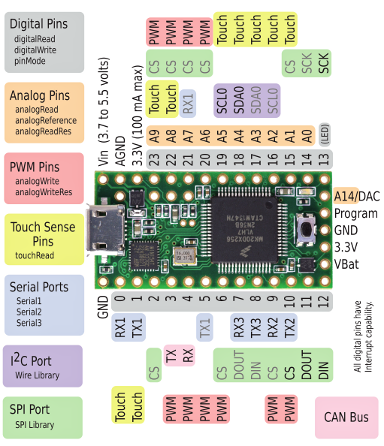
\includegraphics[width=3in]{teensy_pinout.png}
	\caption{Pinout diagram for the Teensy 3.1~\cite{bib:teensy_pinout}.}
	\label{fig:teensy_pinout}
\end{figure}

\begin{figure}[ht]
	\centering
	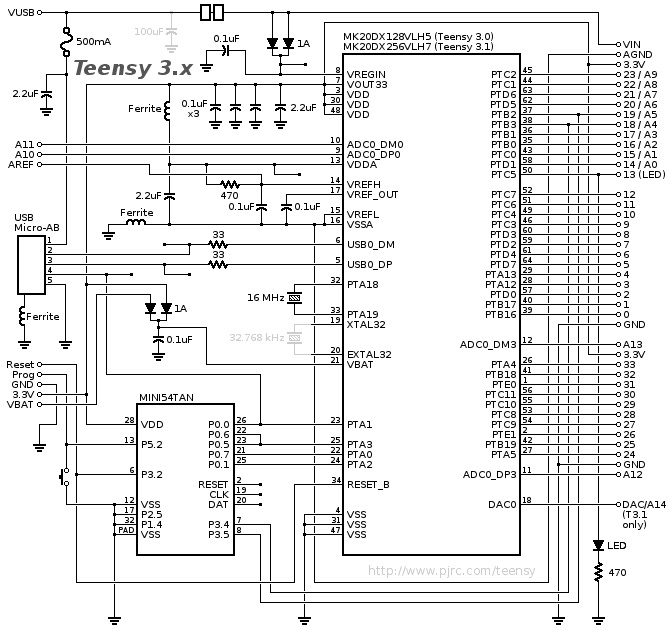
\includegraphics[width=4.5in]{teensy_sch.png}
	\caption{Schematic of the Teensy 3.0/3.1 development platform~\cite{bib:teensy_sch}.}
	\label{fig:teensy_sch}
\end{figure}


The input and output pins of the Teensy are arranged in two parallel rows with a spacing that is compatible with most breadboards. This makes it quite easy to prototype a project where the rest of the components are connected on a breadboard.

The designer of the Teensy platform, Paul J.~Stoffregen, is also an avid software developer. Besides designing the hardware of the Teensy board, he also wrote the software libraries to make the Teensy compatible with the Arduino IDEs, which contributes greatly to the popularity of the Teensy platform. 

To start using the Teensy 3.1, following the instructions at the PJRC website: \url{https://www.pjrc.com/teensy/td_download.html}.


\section{Microcontroller basics}
A microcontrollers is a small computer with all its components, such the processor, memory, and input/output (I/O) interfaces, designed and fabricated on a single integrated circuit (IC). Compared to general purpose computers, a microcontroller usually works at a much lower clock frequency, ranging anywhere between a few kHz to about \SI{200}{\mega\hertz}. The amount of memory available to a microcontroller is also very limited and could be as small as a few kilobyte. Because of the hardware constraints, microcontrollers are usually programmed  us A great advantage of using a microcontroller is its very low power consumption. Some microstrollers need only a few mW of power to run at full speed and even less when stand-by mode. 

The Teensy 
Further reading~\cite{bib:uC_intro1, bib:uC_intro2}.

\section{Lighting up an LED}
Blinking a Light Emitting Diode (LED) is a canonical example in the embedded system world that shares a same popularity as the ``Hello World!'' does in computer programming. There are many ways to turn an LED on and off. The simplest among them is to use a digital output pin to apply the necessary voltage across the LED\footnote{An LED is basically a diode that can emit light when forward biased (anode at a higher electric potential than cathode). The colors of the emitted light of an LED depends on the material composition and the structure of the diode design. The forward voltage drop will also be different for LEDs with different colors.}. 

On the Teensy 3.1, when a pin is set to ``digital high'', it can source some current and its voltage is roughly equal to $VDD$ (in the range of \SIrange{1.7}{3.6}{\volt}). Because of the exponential I-V relationship of the diode, such a large voltage drop across the LED will induce a lot of current, in fact much more than the output circuits in Teensy can handle. Usually a resistor is added to the circuit to prevent this from happening. Similar to a lot of popular microcontroller development platforms, the Teensy has already included an LED with a suitable resistor. If you look at Fig.~\ref{fig:teensy_sch} closely, you will see that an LED and a \SI{470}{\ohm} resistor are connected to pin 13 which is unequivocally labeled as ``LED''. 

So to implement our blinking LED example, we don't actually need to build any circuit. All we need to do is to input the following program\footnote{The program can be accessed through the Arduino IDE by going to ``File-\textgreater Examples-\textgreater Basics-\textgreater Blink''}, compile, and upload to the Teensy. The code is pretty self-explanatory with the added comments. 

\begin{lstlisting}[language=C]

	// LED is connected to pin 13
	int led = 13;
	
	// the setup routine initializes the program
	// it runs once when you press reset. 
	void setup() {                
	// the pinMode routine set up the function of a pin
	// it must be called before a pin can be used as either an input or output device
	pinMode(led, OUTPUT);     
	}
	
	// the loop routine runs over and over again forever:
	void loop() {
	// the digitalWrite routine writes a logic HIGH or LOW value to a digital pin
	// On the Teensy 3.1, a logic HIGH output has a minimum value of (VDD-0.5) V and a logic LOW has a maximum value of 0.5 V.
	digitalWrite(led, HIGH);   // turn the LED on (HIGH is the voltage level)
	delay(1000);               // wait for a second
	digitalWrite(led, LOW);    // turn the LED off by making the voltage LOW
	delay(1000);               // wait for a second
	}
\end{lstlisting}

Here is the Teensy board in action. Unfortunately you can't really see the LED blink. 


\section{Reading digital input}

\section{Using PWM for analog output}

\section{Using interrupts}

Another reason for using interrupts is to ensure the response time for certain tasks. Microcontrollers are used a lot in industrial control systems, where certain sensor inputs must be attended to within a predescribed amount of time to ensure the stability of the control algorithm. Through dedicated hardware, an interrupt triggers the microcontroller to halt the less important task in order to take care of high priority tasks in a timely fashion.

\section{Using the timer}

\section{Using the digital to analog converter (DAC)}

\section{Using the EEPROM}

\section{Using the analog to digital converter (ADC)}

\section{Using the audio library}


\begin{thebibliography}{9}

\bibitem{bib:mk20_ds}
Freescale Semiconductor, Inc., ``K20 Sub-Family Data Sheet'', available: \url{https://www.pjrc.com/teensy/K20P64M72SF1.pdf}, accessed Jun.~24, 2015.

\bibitem{bib:mk20_rm}
Freescale Semiconductor, Inc., ``K20 Sub-Family Reference Manual'', available: \url{https://www.pjrc.com/teensy/K20P64M72SF1RM.pdf}, accessed Jun.~25, 2015.

\bibitem{bib:teensy_sch}
  PJRC.com, LLC, ``Teensy reference: schematic'', online: \url{https://www.pjrc.com/teensy/schematic.html}, accessed Jun.~23, 2015.

\bibitem{bib:teensy_pinout}
  PJRC.com, LLC, ``Teensy: pinouts'', online: \url{https://www.pjrc.com/teensy/teensy31.html}, accessed Jun.~23, 2015.

\bibitem{bib:uC_intro1}
Milan Verle, ``Chapter 1: Introduction to Microcontrollers,'' \emph{Architecture and programming of 8051 MCU's}, online: \url{http://www.mikroe.com/chapters/view/64/chapter-1-introduction-to-microcontrollers/}, accessed Jun.~24, 2015.

\bibitem{bib:uC_intro2}
Gunther Gridling and Bettina Weiss, ``Introduction to Microcontrollers,'' \emph{Courses 182.064 \& 182.074}, Institute of Computer Engineering, Vienna University of Technology, Feb.~26, 2007.


\end{thebibliography}

\end{document}